We present world averages of a selection of \mtau lepton quantities lepton
that most benefit from the adoption of the HFAG
methodology~\cite{Amhis:2012bh}.
All published statistical correlations are used, and a
selection of measurements, particularly the most precise and the most
recent, were studied to take into account the significant systematic
dependencies from external parameters and common systematic sources.

Particular care has been used to engineer a global fit of the \mtau
branching fractions (Section~\ref{sec:tau:br-fit}) to obtain consistent
and statistically complete information for further elaboration in order to
compute lepton universality tests (Section~\ref{sec:tau:leptonuniv}) and
the CKM matrix element $|V_{us}|$ (Section~\ref{sec:tau:vus}).

Finally, we report in Section~\ref{sec:tau:lfv} the most up-to-date limits
on the lepton-flavour-violating \mtau branching fractions and, starting with
this report, we also provide combined upper limits.

%% ///////////////////////////////////////////////////////////////////////////
\tausection{Branching fractions fit}
\cutname{br-fit.html}
\label{sec:tau:br-fit}

The measurements listed in Table~\ref{tab:tau:br-fit} have been used in a
minimum \chisq fit subject to the constraints that are listed
either in the same table (where some fitted quantities and experimental
measurements are expressed as ratios of fit quantities) or in
Section~\ref{sec:tau:constraints}. The fitted quantities and the measurements
are labelled using the PDG $\Gamma_{n}$ notation, where $n$ is
an integer number, which matches the PDG notation for $n<800$. We use
$n\ge 800$ to denote some additional branching fractions, as documented in the
former HFAG report~\cite{Amhis:2012bh}. The PDG $\Gamma_{n}$ notation does
not maintain the same numbers across editions. We continue using the PDG
2010~\cite{PDG_2010} numbers with the aim to eventually switch to a different stable notation,
probably based on PDG identifiers~\cite{pdg-identifiers-2014}.

The fitted branching fractions consist on \htuse{BaseQuantNum} ``base nodes'' and \htuse{ConstrNum} derived
branching fractions, described either as sum of base nodes (see
Section~\ref{sec:tau:constraints}) or as ratios of branching fractions (see
Table~\ref{tab:tau:br-fit}). Furthermore, we define (see
Section~\ref{sec:tau:constraints}) $\Gamma_{\text{All}}$ as the sum of all
the base modes, which correspond to all non-overlapping \mtau decay modes,
$\Gamma_{998} = 1 -\Gamma_{\text{All}}$ and $\Gamma_{110} =
\BRF{\tau^-}{X_s^- \nu_\tau}$, which is the total branching fraction of the
tau to modes with the strangeness quantum number equal to one.

The fitted \hfagtau averages are reported in
Table~\ref{tab:tau:br-fit}. The fit has $\chi^2/\text{d.o.f.} = \htuse{Chisq}/\htuse{Dof}$,
corresponding to a confidence level $\text{CL} = \htuse{ChisqProb}$. We use a total of
\htuse{MeasNum} measurements to fit the above mentioned \htuse{QuantNum} quantities.
Although the unitarity constraint is not applied, the fit is statistically
consistent with unitarity, and the unitarity residual is
\htuse{Gamma998.gn} =  \htuse{Gamma998.td} = \htuse{Gamma998}.

In several cases, when it is statistically equivalent within the \hfagtau
fitting procedure, for historical reasons the statistical and systematic
errors are added in quadrature and are reported in the above table in the
location of the statistical error, reporting zero as systematic error. A
scale factor of 5.44 (as in the two previous reports
report~\cite{Asner:2010qj,Amhis:2012bh}) has been applied to the published
uncertainties of the two severely inconsistent measurements of
\(\Gamma_{96} = \tau \to KKK\nu\) by \babar and Belle, following the same
procedure as the PDG.

\tausubsection{Changes with respect to the previous report}

The following additions and changes gave been done with respect to the 2012
report~\cite{Amhis:2012bh}.

Published results from two \babar papers and one Belle paper have been
added. The following results have been used from the \htuse{LEES 2012X.collab} high
multiplicity decay \mtau branching fractions paper~\htuse{LEES 2012X.cite}:
{\setlength{\LTleft}{\parindent}%
\begin{longtable}{@{}ll@{}}
\htuse{LEES 2012X.meas}.
\end{longtable}}
\noindent These results superseed the previous \babar results $\tau^- \to
\htuse{Gamma136.td}$~\cite{Aubert:2008nj} and $\tau^- \to
\htuse{Gamma103.td}$~\cite{Aubert:2005waa}. The following
results have been used from the \htuse{LEES 2012Y.collab} paper on the
\mtau branching fractions with two
$K_S$~\htuse{LEES 2012Y.cite}:
{\setlength{\LTleft}{\parindent}%
\begin{longtable}{@{}ll@{}}
\htuse{LEES 2012Y.meas},
\end{longtable}}
\noindent The following results have been used from the
\htuse{Ryu:2014vpc.collab} paper on the $K_S$ final
states~\htuse{Ryu:2014vpc.cite}:
{\setlength{\LTleft}{\parindent}%
\begin{longtable}{@{}ll@{}}
\htuse{Ryu:2014vpc.meas},
\end{longtable}}
\noindent these results supersede the preliminary ones~\cite{Ryu:2012pm}
and the former published result on $\tau^- \to \htuse{Gamma35.td}$~\cite{Epifanov:2007rf}.
In order to profit from the measurements of branching fractions with two
$K_S$ in the final state, we discard the inclusive ALEPH measurement on
$\tau^- \to \htuse{Gamma49.td}$~\cite{Barate:1999hj} and we add the exclusive ALEPH
measurement on $\tau^- \to \htuse{Gamma51.td}$~\cite{Barate:1999hj}.

The CLEO result on  $\tau^- \to \htuse{Gamma136.td}$~\cite{Anastassov:2000xu}
has been discarded since it is very correlated with the branching fractions
into six pions measured in the same paper, which are dominated by the $\eta$ and
$\omega$ resonances.

We added the $\tau^- \to \htuse{Gamma128.td}$ measurements by CLEO~\cite{Bartelt:1996iv}
and ALEPH~\cite{Buskulic:1996qs} to complete the list of useful experimental inputs for
this mode.

In order to best integrate the above new results in the global fit, the following
constraints have been added:
{\setlength{\LTleft}{\parindent}%
\begin{tabularx}{\linewidth-\parindent}{@{}lX@{}}
  \htuse{Gamma13.c.constr.eq} \\
  \htuse{Gamma33.c.constr.eq} \\
  \htuse{Gamma49.c.constr.eq} \\
  \htuse{Gamma78.c.constr.eq} \\
  \htuse{Gamma103.c.constr.eq} \\
  \htuse{Gamma104.c.constr.eq} \\
  \htuse{Gamma806.c.constr.eq} \\
  \htuse{Gamma810.c.constr.eq} \\
  \htuse{Gamma820.c.constr.eq} \\
  \htuse{Gamma830.c.constr.eq} \\
  \htuse{Gamma910.c.constr.eq} \\
  \htuse{Gamma930.c.constr.eq} \\
  \htuse{Gamma944.c.constr.eq} \\
\end{tabularx}}
\noindent It was realised that the \htuse{Gamma44.gn} fit quantity, which is
exclusively determined by one single ALEPH
result~\htuse{ALEPH.Gamma44.pub.BARATE.99R,ref}, does actually exclude the
contribution from $K^0\to\pi^0\pi^0$, so we renamed it to
$\htuse{Gamma44.gn} = \htuse{Gamma44.td}$.
The definition of the total branching fraction and of the inclusive
branching fraction of the \mtau lepton into a strange final states have
been updated as follows:
{\setlength{\LTleft}{\parindent}%
\begin{tabularx}{\linewidth-\parindent}{@{}lX@{}}
  \htuse{Gamma110.c.constr.eq} \\
  \htuse{GammaAll.c.constr.eq}~.
\end{tabularx}}
\noindent The total \mtau branching fraction \htuse{GammaAll.gn} definition
includes two modes that have overlapping final states, to a minor extent:
\begin{align*}
  &\htuse{Gamma50.gn} =  \htuse{Gamma50.td}~, \\
  &\htuse{Gamma132.gn} =  \htuse{Gamma132.td}~.
\end{align*}
\noindent The amount of overlap cannot be disentagled with the presently
available measurements, however we consider it negligible since the
involved branching fractions are small and their overlap is conceivably minor.
A wrong constraint used in the two previous reports has been
removed:
{\setlength{\LTleft}{\parindent}%
\begin{tabularx}{\linewidth-\parindent}{@{}lX@{}}
  $\Gamma_{136}$ ={}& $\Gamma_{104}\cdot \Gamma_{\eta \to \pi^+\pi^-\pi^0} +
  \Gamma_{78} \cdot \Gamma_{\eta \to 3\pi^0}$~.
\end{tabularx}}
\noindent The wrong constraint has been affecting in a negligible way the
global fit in the previous HFAG reports, except for the involved specific
branching ratios.  In particular, the effects on the lepton universality
tests and in the \Vus determination were negligible.

Finally, the constraint parameters (see Section~\ref{sec:tau:constraints})
have been updated to the PDG 2013 results~\cite{PDG_2012}.

%%
%% quantities and measurements
%%
\begin{center}
\begin{envsmall}
\setlength{\LTcapwidth}{0.85\linewidth}
\renewcommand*{\arraystretch}{1.3}%
\ifhevea
\renewcommand{\bar}[1]{\textoverline{#1}}
\else
\begin{citenoleadsp}
\fi
\begin{longtable}{llll}
\caption{HFAG \hfagTauTag branching fractions fit results.\label{tab:tau:br-fit}}%
\\
\hline
\multicolumn{1}{l}{\bfseries \mtau lepton branching fraction} &
\multicolumn{1}{l}{\bfseries Fit value / Exp.} &
\multicolumn{1}{l}{\bfseries HFAG Fit / Ref.} \\
\hline
\endfirsthead
\multicolumn{4}{c}{{\bfseries \tablename\ \thetable{} -- continued from previous page}} \\ \hline
\multicolumn{1}{l}{\bfseries \mtau lepton branching fraction} &
\multicolumn{1}{l}{\bfseries Fit value / Exp.} &
\multicolumn{1}{l}{\bfseries HFAG Fit / Ref.} \\
\hline
\endhead
\endfoot
\endlastfoot
\htuse{BrVal} \\
\hline
\end{longtable}
\ifhevea\else
\end{citenoleadsp}
\fi
\end{envsmall}
\end{center}

\tausubsection{Correlation between base nodes uncertainties}
\label{sec:tau:fitcorr}

The following tables report the correlation coefficients between base nodes,
in percent.

%%
%% base nodes correlations
%%
\htuse{BrCorr}

\tausubsection{Equality constraints}
\label{sec:tau:constraints}

We use equality constraints that relate a branching fraction to a sum of
branching fractions. As mentioned above, the \mtau branching fractions are
denoted with $\Gamma_n$ labels. In the constraint relations we use the
values of some non-tau branching fractions, denoted e.g.\ with the
self-describing notation $\Gamma_{K_S \to \pi^0\pi^0}$. We also use
probabilities corresponding to modulus square amplitudes describing quantum
mixtures of states such as $K^0$, $\bar{K}^0$, $K_S$, $K_L$, denoted with
e.g.\ $\Gamma_{<K^0|K_S>} = |{<}K^0|K_S{>}|^2$.
In the fit, all non-tau quantities are taken from the PDG 2013~\cite{PDG_2012}
fits (when available) or averages, and are used without accounting for their
uncertainties, which are however in general small with respect
to the uncertainties on the \mtau branching fractions.
The \mtau branching fractions are illustrated in Table~\ref{tab:tau:br-fit}.
The equations in the following permit the computation of the values and
uncertainties for branching fractions that are not listed in
Table~\ref{tab:tau:br-fit}, once they are expressed as function of the
quantities that are listed there. The following list does not include the
(non-linear) constraints already introduced in
Section~\ref{sec:tau:br-fit}, and illustrated in
Table~\ref{tab:tau:br-fit}, where some measured branching fractions are
expressed as ratios of ``base'' branching fractions.

\begin{envsmall}
  \setlength\abovedisplayskip{0pt}
  \setlength\belowdisplayshortskip{0pt}
  \ifhevea\renewcommand{\bar}[1]{\textoverline{#1}}\fi
  %%
  %% after editing content of \htuse{ConstrVal} macro for better formatting
  %%
  \htuse{ConstrEqs}
\end{envsmall}

\tausubsection{Fit procedure}
\label{sec:tau:fit}

The fit procedure is functionally equivalent to the one employed in the
former HFAG reports~\cite{Asner:2010qj,Amhis:2012bh} and consists in a minimum \chisq
fit subject to linear and non-linear constraints.

\tausection{\mtau lifetime average}
\cutname{lifetime.html}
\label{sec:tau:lifetime}

The recent Belle \mtau lifetime measurement has
reduced the world average uncertainty by a factor two. The HFAG-Tau average
is equivalent to the PDG 2014 average~\cite{PDG_2014} (see Fig.~\ref{fig:tau:tau-lifetime}).
\begin{figure}[tb]
  \begin{center}
   \ifhevea
    \begin{tabular}{@{}cc@{}}
      \larger\bfseries\ahref{plot-taulife-hfag-summer2014.png}{PNG format} &
      \larger\bfseries\ahref{plot-taulife-hfag-summer2014.pdf}{PDF format} \\
      \multicolumn{2}{c}{\ahref{plot-taulife-hfag-summer2014.png}{%
          \imgsrc[alt="Vus summary plot"]{plot-taulife-hfag-summer2014.png}}}
    \end{tabular}
    \else
    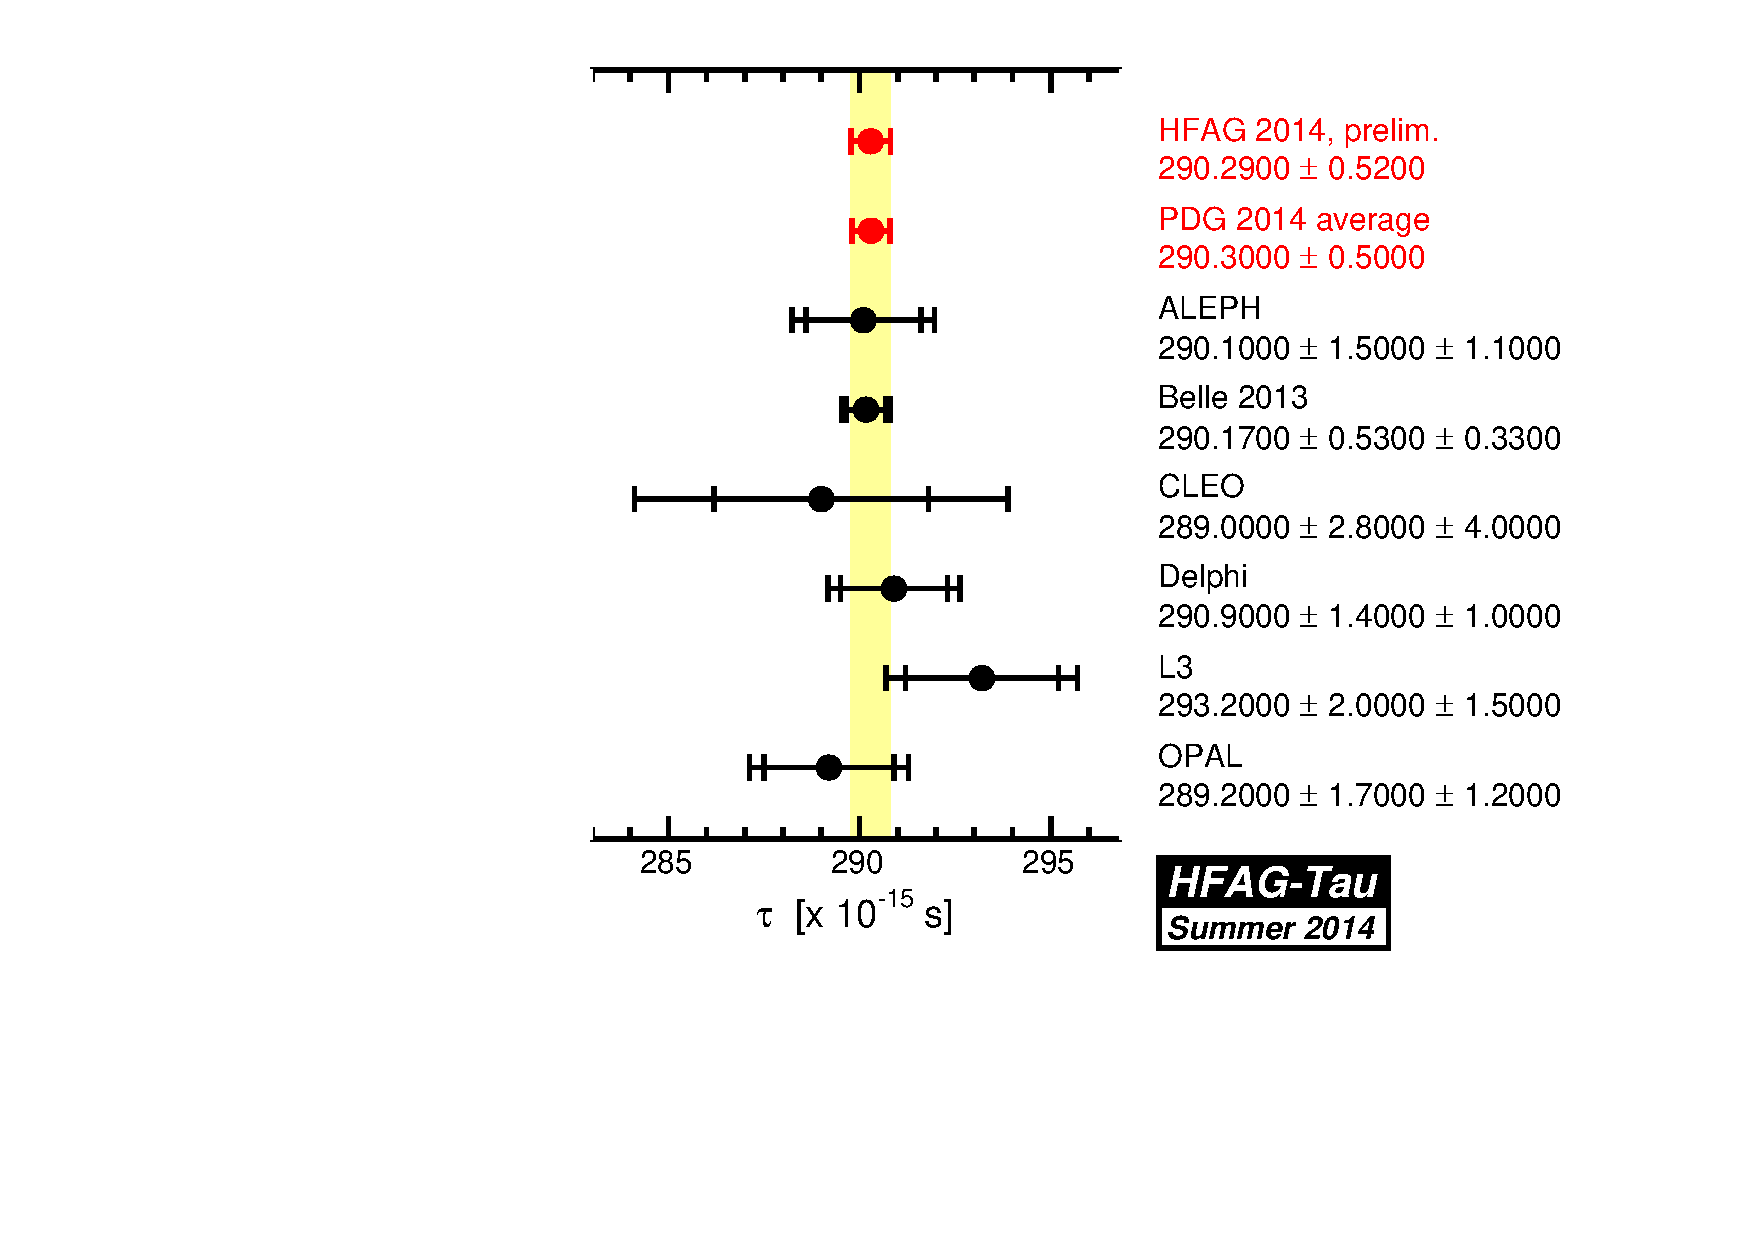
\includegraphics[width=0.75\linewidth,clip]{figures/tau/plot-taulife-hfag-summer2014.pdf}
    \fi
    \caption{\mtau lifetime average.%
      \label{fig:tau:tau-lifetime}%
    }
  \end{center}
\end{figure}

%% ///////////////////////////////////////////////////////////////////////////
\tausection{Tests of lepton universality}
\cutname{lepton-univ.html}
\label{sec:tau:leptonuniv}

Lepton universality tests precision has significantly been improved by the
addition of the recent Belle \mtau lifetime
measurement~\cite{Belous:2013dba}, while improvements from the \mtau
branching fraction fit are negligible.
We compute the universality tests like in the previous report by using
proper ratios of the partial widths of a heavier lepton \lepth
decaying to a
lighter lepton \leptl~\cite{Marciano:1988vm},
\begin{align*}
  \Gamma(\lepth \to \nu_{\lepth} \leptl \nub_{\leptl} (\gamma)) =
  \frac{\BR(\lepth \to \nu_{\lepth} \leptl \nub_{\leptl})}{\tau_{\lepth}} =
  \frac {G_{\lepth} G_{\leptl} m^5_{\lepth}}{192 \pi^3}\, f\left(\frac {m^2_{\leptl}}{m^2_{\lepth}}\right)
  \opdelta^{\lepth}_W \opdelta^{\lepth}_\gamma~,
\end{align*}
where
\begin{alignat*}{3}
 G_{\leptl} &= \frac {g^2_{\leptl}}{4 \sqrt{2} M^2_W} &\quad&&
 f(x) &= 1 -8x +8x^3 -x^4 -12x^2 \text{ln}x \\
 \opdelta^{\lepth}_W &= 1 + \frac {3}{5} \frac {m^2_{\lepth}}{M^2_W} &\quad\quad&&
 \opdelta^{\lepth}_\gamma &= 1+\frac {\alpha(m_{\lepth})}{2\pi} \left(\frac {25}{4}-\pi^2\right)
\end{alignat*}
We use $\opdelta^\tau_\gamma=1-43.2\cdot 10^{-4}$ and
$\opdelta^\mu_\gamma=1-42.4\cdot 10^{-4}$~\cite{Marciano:1988vm} and $M_W$
from PDG 2013~\cite{PDG_2012}.
We use HFAG 2014 averages and PDG 2013 for the other quantities.
Using pure leptonic processes we obtain
\begin{align*}
  \left( \frac{g_\tau}{g_\mu} \right) = \htuse{gtaubygmu_tau}~,
  && \left( \frac{g_\tau}{g_e} \right) = \htuse{gtaubyge_tau}~,
  && \left( \frac{g_\mu}{g_e} \right) = \htuse{gmubyge_tau}~.
\end{align*}
Using semi-hadronic processes
\begin{align*}
  \left( \frac{g_\tau}{g_\mu} \right)^2 =
  \frac{\BR({\tau \to h \nu_\tau})}{\BR({h \to \mu \bar{\nu}_\mu})}
  \frac{2m_h m^2_{\mu}\tau_h}{(1+\delta_{h})m^3_{\tau}\tau_{\tau}}
  \left( \frac{1-m^2_{\mu}/m^2_h}{1-m^2_h/m^2_{\tau}} \right)^2~,
\end{align*}
where $h$ = $\pi$ or $K$ and the radiative corrections are
$\delta_{\pi} = (\htuse{delta_LD_taupi_pimu})\%$ and
$\delta_{K} = (\htuse{delta_LD_tauK_Kmu})\%$~\cite{Decker:1994dd}.
we measure:
\begin{align*}
  \left( \frac{g_\tau}{g_\mu} \right)_\pi &= \htuse{gtaubygmu_pi}~,
  & \left( \frac{g_\tau}{g_\mu} \right)_K = \htuse{gtaubygmu_K}~.
\end{align*}
Similar tests could be performed with decays to electrons, however they are
less precise because the hadron two body decays to electrons are
helicity-suppressed.
Averaging the three \(g_\tau/g_\mu\) ratios we obtain
\begin{align*}
  \left( \frac{g_\tau}{g_\mu} \right)_{\tau{+}\pi{+}K} &= \htuse{gtaubygmu_fit}~,
\end{align*}
accounting for statistical correlations.
Table~\ref{tab:tau:univ-fit-corr} reports the statistical correlation coefficients for the fitted coupling ratios:
\ifhevea\begin{table}\fi%% otherwise cannot have normalsize caption
\begin{center}
\ifhevea
\caption{Universality coupling ratios correlation coefficients (\%)\label{tab:tau:univ-fit-corr}}%
\else
\begin{minipage}{\linewidth}
\begin{center}
\captionof{table}{Universality coupling ratios correlation coefficients (\%)}\label{tab:tau:univ-fit-corr}%
\fi
\begin{center}
\renewcommand*{\arraystretch}{1.1}%
\begin{tabular}{lcccc}
\toprule
\htuse{couplingsCorr}
\\\bottomrule
\end{tabular}
\end{center}
\ifhevea\else
\end{center}
\end{minipage}
\fi
\end{center}
\ifhevea\end{table}\fi

%% ///////////////////////////////////////////////////////////////////////////
\tausection{Universality improved $\BR(\tau \to e \nu \bar{\nu})$ and $\Rhad$}
\cutname{Be_univ_and_Rtau.html}
\label{sec:tau:be-univ-rtau}

Following Ref.~\cite{Davier:2005xq}, we assume lepton universality to
obtain a more precise experimental determination of $\BR_e = \BR(\tau \to
e\bar{\nu}_e\nu_\tau)$ using the \mtau branching fraction to muon and the \mtau
lifetime. We average:
\begin{itemize}

\item the $\BR_e$ fit value,

\item the $\BR_e$ determination from $\BR_\mu$ assuming that
$g_\mu/g_e = 1$ hence (see also Section~\ref{sec:tau:leptonuniv})
$\BR_e = \BR_\mu \cdot f(m^2_e/m^2_\tau)/f(m^2_\mu/m^2_\tau)$,

\item the $\BR_e$ determination from the \mtau lifetime assuming that
$g_\tau/g_\mu =1$ hence $\BR_e = \BR(\mu \to e \bar{\nu}_e
\nu_\mu)\cdot (\tau_\tau / \tau_\mu) \cdot (m_\tau/m_\mu)^5 \cdot
f(m^2_e/m^2_\tau)/f(m^2_e/m^2_\mu) \cdot (\delta_\gamma^\tau
\delta_W^\tau)/(\delta_\gamma^\mu \delta_W^\mu)$ where $\BR(\mu \to e
\bar{\nu}_e \nu_\mu) = 1$.

\end{itemize}
Accounting for statistical correlations, we obtain
\begin{align*}
  \BR_e^{\text{uni}} = (\htuse{Be_univ})\%.
\end{align*}
The recent Belle \mtau lifetime measurement has brought a significant improvement.
We use $\BR_e^{\text{uni}}$ to obtain the ratio
\begin{align*}
  \Rhad = \frac{\Gamma(\tau \to \text{hadrons})}{\Gamma(\tau\to e\nu\bar{\nu})} = \htuse{R_tau}.
\end{align*}
Here $\Gamma(\tau \to \text{hadrons})$ is obtained by summing all \mtau
hadronic decay modes.

%% ///////////////////////////////////////////////////////////////////////////
\tausection{$\Vus$ measurement}
\cutname{vus.html}
\label{sec:tau:vus}

We have updated the CKM coefficient \Vus determinations of the previous
report using the updated data from HFAG 2014 and PDG 2013.

\tausubsection{Inclusive \mtau partial width to strange}

The \mtau hadronic partial width is the sum of the \mtau partial width to
strange and to non-strange hadronic final states,
$\Gammahad = \Gammastrange + \Gammanonstrange$.
Dividing by the partial width to electron, $\Gamma_e$, we obtain partial width ratios
(which are equal to the respective branching fraction ratios) for which
$\Rhad =  \Rstrange + \Rnonstrange$. In terms
of such ratios, \Vus is measured as
\begin{align*}
  \Vus &= \sqrt{\Rstrange/\left[\frac{\Rnonstrange}{\Vud^2} -  \delta R_{\text{theory}}\right]}~,
\end{align*}
where $\delta R_{\text{theory}}$ can be determined in the context of low
energy QCD theory, partly relying on experimental low energy scattering
data. The literature reports several
calculations~\cite{Gamiz:2006xx,Gamiz:2007qs,Maltman:2010hb}. In this
report we use Ref.~\cite{Gamiz:2006xx}, whose estimated uncertainty size is
in between the two other ones. We use the information in that paper and the
PDG 2013 value for the $s$-quark mass $m_s = \htuse{m_s}$~\cite{PDG_2012}
to calculate $\delta R_{\text{theory}} = \htuse{deltaR_su3break}$.

We proceed following the same procedure of the 2012 HFAG
report~\cite{Amhis:2012bh}, using the universality improved $\BR_e^{\text{uni}}$
(see Section~\ref{sec:tau:be-univ-rtau}) to compute the $R$ ratios, and
using the sum of the \mtau branching fractions to strange and
non-strange hadronic final states to compute \Rstrange and \Rnonstrange,
respectively.

Using the \mtau branching fraction fit results with their uncertainties
and correlations (Section~\ref{sec:tau:br-fit}), we compute $\BRstrange =
(\htuse{B_tau_s_fit})\%$ (see also Table~\ref{tab:tau:vus}) and
$\BRnonstrange = (\htuse{B_tau_VA_fit})\%$. PDG 2013 averages
are used for non-\mtau quantities, including $\Vud = \htuse{Vud}$, which
comes from Ref.~\cite{Hardy:2008gy} like for the previous HFAG report.

We obtain $\VusTauIncl = \htuse{Vus}$, which
is $\htuse{Vus_mism_sigma_abs}\sigma$ lower than the unitarity CKM
prediction $\VusUni = \htuse{Vus_uni}$, from $(\VusUni)^2 = 1 -
\Vud^2$. The \VusTauIncl uncertainty includes a systematic error
contribution of \htuse{Vus_err_th_perc}\% from the theory uncertainty on
$\delta R_{\text{theory}}$. There is no significant change with respect to
the previous HFAG report.

Kim Maltman has computed an alternative theoretical estimate based on Fixed
Order Pertubation Theory and experimental inputs restricted to \mtau
quantities. 
The result is  $\delta R_{\text{theory}} = 0.254 \pm 0.038$~\cite{Maltman:oct2014}.
The uncertainty includes an additional contribution to account
for the differences between using Fixed Order Pertubation Theory and Contour
Improved Perturbation Theory. With this alternative value, we would obtain
$\VusTauIncl = 0.2181 \pm 0.0022$, which would be $3.1\sigma$ lower than
the unitarity CKM prediction.

%%
%% Gamma110 quantities
%%
\begin{table}
\begin{center}
\renewcommand*{\arraystretch}{1.3}%
\caption{HFAG \hfagTauTag \mtau branching fractions to strange final states.\label{tab:tau:vus}}%
\ifhevea\renewcommand{\bar}[1]{\textoverline{#1}}\fi
\begin{envsmall}
\begin{center}
\begin{tabular}{llll}
\hline
\multicolumn{1}{c}{\bfseries Branching fraction} &
\multicolumn{1}{c}{\bfseries HFAG \hfagTauTag fit} \\
\hline
\htuse{BrStrangeVal}
\\\hline
\htuse{BrStrangeTotVal}
\\\hline
\end{tabular}
\end{center}
\end{envsmall}
\end{center}
\end{table}

\tausubsection{\Vus from $\BR(\tau \to K\nu) / \BR(\tau \to \pi\nu)$ and from $\BR(\tau \to K\nu)$}

We follow the same procedure of the HFAG 2012 report to compute \Vus from
the ratio of branching fractions $\BFtautoknu/\BFtautopinu =
\htuse{Gamma10by5}$ from the equation
\begin{align*}
\frac{\BFtautoknu}{\BFtautopinu} &=
\frac{f_K^2 \Vus^2}{f_\pi^2 \Vud^2} \frac{\left( 1 - m_K^2/m_\tau^2 \right)^2}{\left( 1 -  m_\pi^2/m_\tau^2 \right)^2}
\frac{\opdelta_{\text{LD}}(\tau^- \to K^-\nut)}{\opdelta_{\text{LD}}(\tau^- \to \pi^-\nut)}~.
\end{align*}
We use $f_K/f_\pi = \htuse{f_K_by_f_pi}$ from the
FLAG 2013 Lattice averages with $N_f=2+1$~\cite{Aoki:2013ldr}.
We compute $\VusTauKpi = \htuse{Vus_tauKpi}$,
$\htuse{Vus_tauKpi_mism_sigma_abs}\sigma$ below the CKM unitarity prediction.

We proceed like in 2012 also to determine \Vus from the branching fraction
$\BFtautoknu$ using
\begin{align*}
  \BR(\tau^- \to K^-\nu_\tau) =
  \frac{G^2_F f^2_K \Vus^2 m^3_{\tau} \tau_{\tau}}{16\pi\hbar} \left (1 - \frac{m_K^2}{m_\tau^2} \right )^2 S_{EW}~.
\end{align*}
We use $f_K = \htuse{f_K}\,\mev$ from FLAG 2013 with
$N_f=2+1$~\cite{Aoki:2013ldr}. We obtain $\VusTauKnu = \htuse{Vus_tauKnu}$,
which is $\htuse{Vus_tauKnu_mism_sigma_abs}\sigma$ below
the CKM unitarity prediction. CODATA 2010 results~\cite{Mohr:2012tt} and
PDG 2013 have been used for the physics constants.

\tausubsection{\Vus from \mtau summary}

\begin{figure}[tb]
  \begin{center}
   \ifhevea
    \begin{tabular}{@{}cc@{}}
      \larger\bfseries\ahref{hfag-tau-vus-plot.png}{PNG format} &
      \larger\bfseries\ahref{hfag-tau-vus-plot.pdf}{PDF format} \\
      \multicolumn{2}{c}{\ahref{hfag-tau-vus-plot.png}{%
          \imgsrc[alt="Vus summary plot"]{hfag-tau-vus-plot.png}}}
    \end{tabular}
    \else
    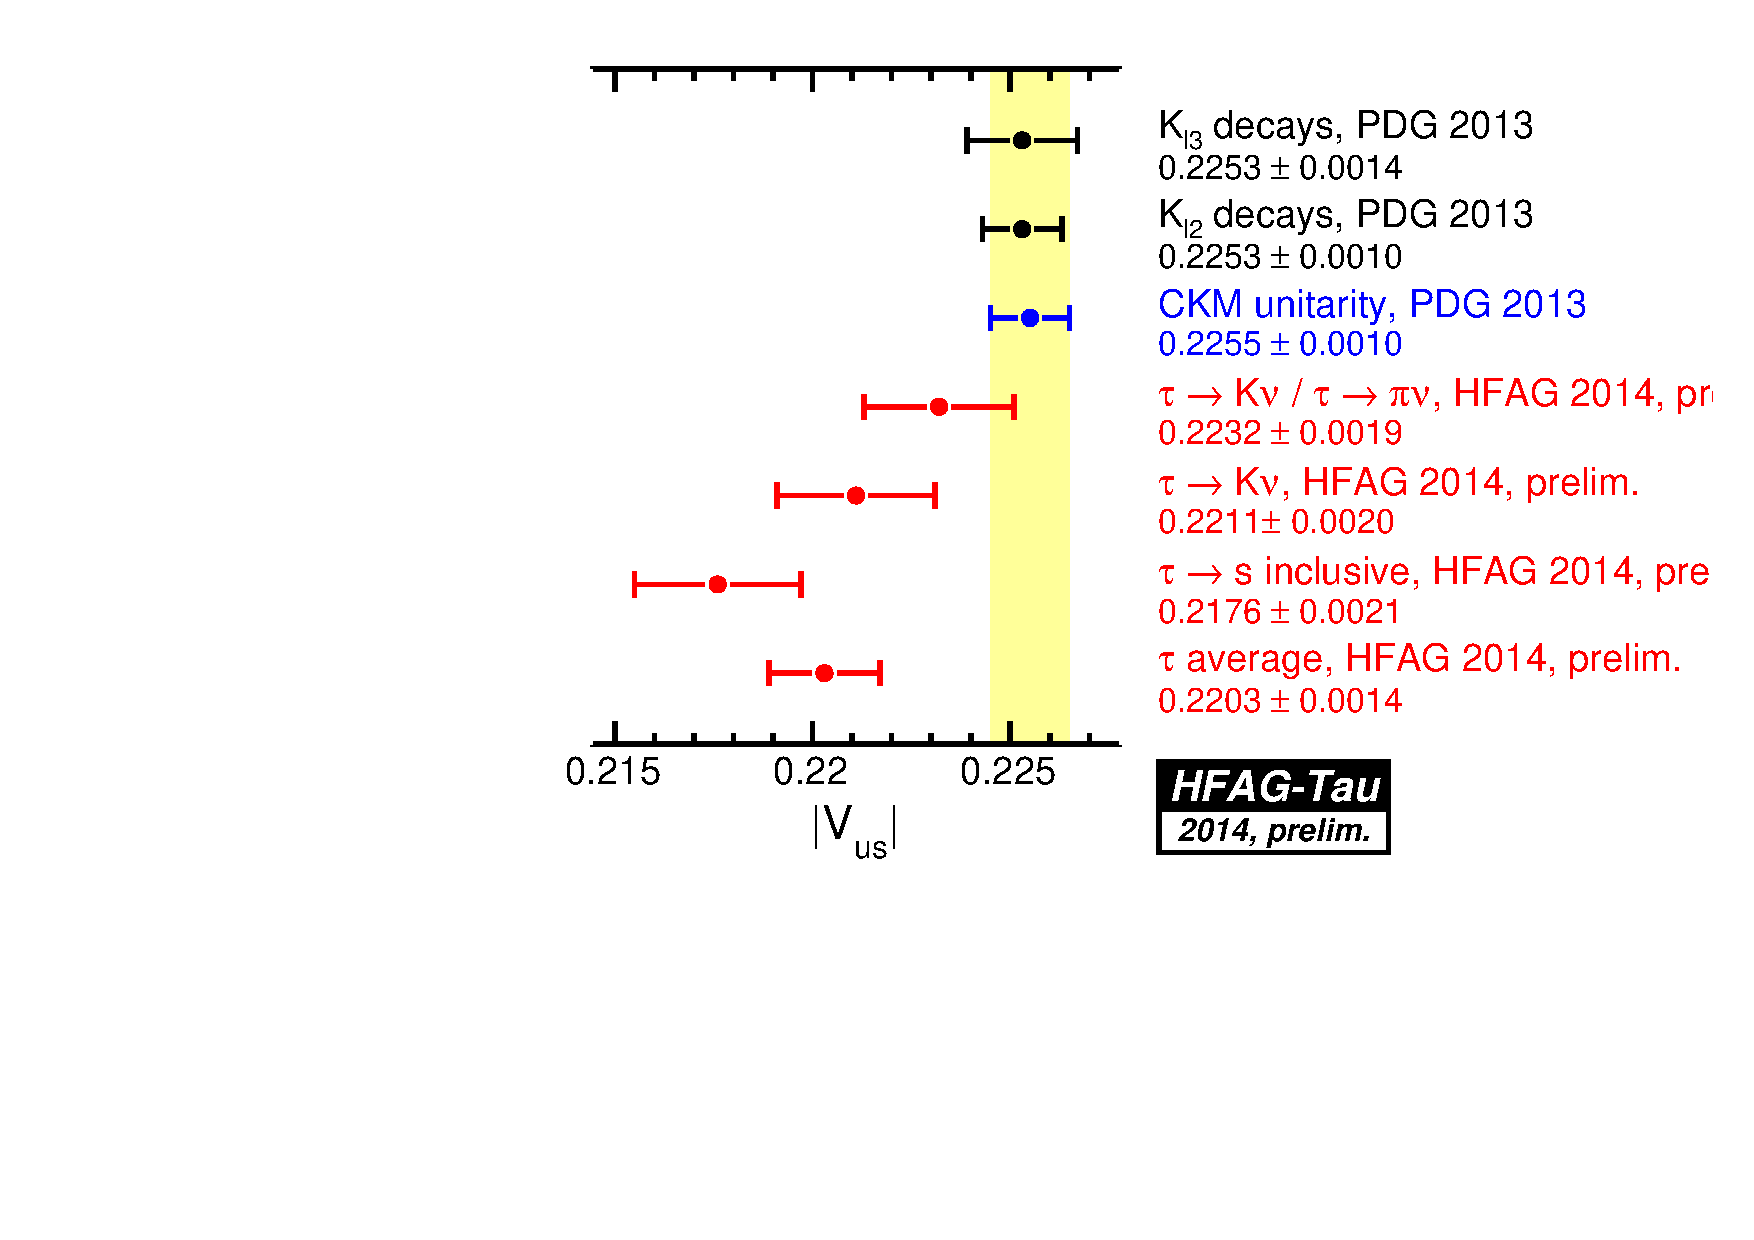
\includegraphics[width=0.75\linewidth,clip]{figures/tau/hfag-tau-vus-plot.pdf}
    \fi
    \caption{\Vus averages of this document compared with the FlaviaNet results~\cite{Antonelli:2010yf}.
      \label{fig:tau:vus-summary}%
    }
  \end{center}
\end{figure}

We summarize the \Vus results reporting the values, the discrepancy with
respect to the \Vus determination from CKM unitarity, and an illustration
of the measurement method:
\begin{alignat*}{6}
  &\VusUni &&= \htuse{Vus_uni} & \quad & & \quad
  & {\smaller\text{from } \sqrt{1 - \Vud^2} \quad\text{(CKM unitarity)}}~, \\
  %%
  &\VusTauIncl &&= \htuse{Vus} & \quad & \htuse{Vus_mism_sigma}\sigma &
  & {\smaller\text{from } \Gamma(\tau^- \to X_s^- \nut)}~, \\
  %%
  &\VusTauKpi &&= \htuse{Vus_tauKpi} & \quad & \htuse{Vus_tauKpi_mism_sigma}\sigma &
  & {\smaller\text{from } \Gamma(\tauknu)/\Gamma(\taupinu)}~,  \\
  %%
  &\VusTauKnu &&= \htuse{Vus_tauKnu} & \quad & \htuse{Vus_tauKnu_mism_sigma}\sigma &
  & {\smaller\text{from } \Gamma(\tauknu)}~.
\end{alignat*}

Averaging the three above \Vus determinations we obtain:
\begin{alignat*}{6}
  & \Vus_\tau &&= \htuse{Vus_tau} &\quad &\htuse{Vus_tau_mism_sigma}\sigma \quad
  & \text{average of 3 \Vus \mtau measurements}.
\end{alignat*}
We could not find a published estimate of the correlation of the
uncertainties on $f_K$ and $f_K/f_\pi$, but even if we assume $\pm
100\%$ correlation, the uncertainty on $\Vus_\tau$ does not change
more than about $\pm 5\%$. Figure~\ref{fig:tau:vus-summary} summarizes the
\Vus results.
